% Complex points z_i (red) and their upper-half square roots w_i (blue).
% Faithful redraw of the Asymptote diagram in book/tex/complex-ana/log.tex.
\documentclass[border=2mm]{standalone}
\usepackage{tikz}\usetikzlibrary{arrows.meta}
\begin{document}
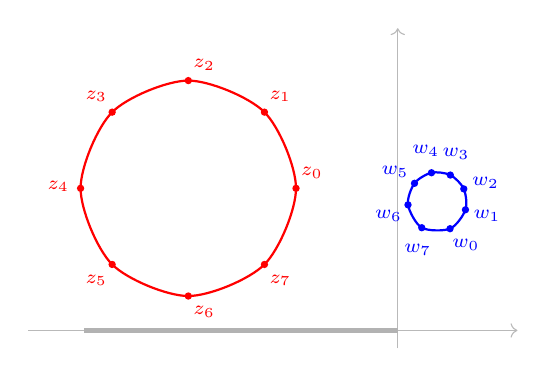
\begin{tikzpicture}[scale=0.95]
  \draw[->,gray!55] (-4.94,0) -- (1.60,0);
  \draw[->,gray!55] (0,-0.24) -- (0,4.04);
  \draw[gray!60,line width=1.6pt] (0,0) -- (-4.20,0);
  \draw[red,thick] plot[smooth cycle] coordinates {(-1.360,1.900) (-1.782,2.918) (-2.800,3.340) (-3.818,2.918) (-4.240,1.900) (-3.818,0.882) (-2.800,0.460) (-1.782,0.882)};
  \fill[red] (-1.360,1.900) circle (1.4pt); \node[red,font=\scriptsize] at (-1.148,2.112) {$z_{0}$};
  \fill[red] (-1.782,2.918) circle (1.4pt); \node[red,font=\scriptsize] at (-1.570,3.130) {$z_{1}$};
  \fill[red] (-2.800,3.340) circle (1.4pt); \node[red,font=\scriptsize] at (-2.588,3.552) {$z_{2}$};
  \fill[red] (-3.818,2.918) circle (1.4pt); \node[red,font=\scriptsize] at (-4.030,3.130) {$z_{3}$};
  \fill[red] (-4.240,1.900) circle (1.4pt); \node[red,font=\scriptsize] at (-4.539,1.926) {$z_{4}$};
  \fill[red] (-3.818,0.882) circle (1.4pt); \node[red,font=\scriptsize] at (-4.030,0.670) {$z_{5}$};
  \fill[red] (-2.800,0.460) circle (1.4pt); \node[red,font=\scriptsize] at (-2.588,0.248) {$z_{6}$};
  \fill[red] (-1.782,0.882) circle (1.4pt); \node[red,font=\scriptsize] at (-1.570,0.670) {$z_{7}$};
  \draw[blue,thick] plot[smooth cycle] coordinates {(0.699,1.360) (0.905,1.613) (0.883,1.892) (0.703,2.077) (0.451,2.108) (0.224,1.967) (0.137,1.679) (0.321,1.373)};
  \fill[blue] (0.699,1.360) circle (1.4pt); \node[blue,font=\scriptsize] at (0.911,1.147) {$w_{0}$};
  \fill[blue] (0.905,1.613) circle (1.4pt); \node[blue,font=\scriptsize] at (1.195,1.535) {$w_{1}$};
  \fill[blue] (0.883,1.892) circle (1.4pt); \node[blue,font=\scriptsize] at (1.172,1.970) {$w_{2}$};
  \fill[blue] (0.703,2.077) circle (1.4pt); \node[blue,font=\scriptsize] at (0.780,2.366) {$w_{3}$};
  \fill[blue] (0.451,2.108) circle (1.4pt); \node[blue,font=\scriptsize] at (0.373,2.398) {$w_{4}$};
  \fill[blue] (0.224,1.967) circle (1.4pt); \node[blue,font=\scriptsize] at (-0.036,2.117) {$w_{5}$};
  \fill[blue] (0.137,1.679) circle (1.4pt); \node[blue,font=\scriptsize] at (-0.123,1.529) {$w_{6}$};
  \fill[blue] (0.321,1.373) circle (1.4pt); \node[blue,font=\scriptsize] at (0.269,1.077) {$w_{7}$};
\end{tikzpicture}\end{document}
